\documentclass{article}

\usepackage[utf8]{inputenc}
\usepackage[english,russian]{babel}
\usepackage[T2A]{fontenc}
\usepackage{tabularx}
\usepackage{amsmath,mathrsfs,amssymb}
\usepackage{bbding}
\usepackage{alltt}
\usepackage{epigraph}
\usepackage{verbatim}
\usepackage{soul}
\usepackage{latexsym}
\usepackage{array}
\usepackage{comment}
\usepackage{makeidx}
\usepackage{listings}
\usepackage{indentfirst}
\usepackage{verbatim}
\usepackage{color}
\usepackage{url}
\usepackage{xspace}
\usepackage{hyperref}
\usepackage{stmaryrd}
\usepackage{tikz}
\usetikzlibrary{arrows,decorations.pathreplacing,backgrounds,fit,positioning,shapes,chains,calligraphy,arrows.meta,shapes.arrows,overlay-beamer-styles}
\usepackage{euscript}
\usepackage{mathtools}
\usepackage{graphicx}
\usepackage{euscript}
\usepackage{mathtools}
\usepackage{transparent}
\usepackage{bold-extra}

\newcommand{\sembr}[1]{\llbracket{#1}\rrbracket}
\newcommand{\primi}[1]{\mathbf{#1}}
\newcommand{\Int}[2]{\primi{int}^{\mathcal {#1}}_{\mathcal {#2}}}
\newcommand{\Sem}[2]{\sembr{#1}_{\mathcal {#2}}}

\newcommand{\lama}{$\lambda\kern -.1667em\lower -.5ex\hbox{$a$}\kern -.1000em\lower .2ex\hbox{$\mathcal M$}\kern -.1000em\lower -.5ex\hbox{$a$}$\xspace}
\sloppy

\lstdefinelanguage{cc}{
basicstyle=\ttfamily\small,
keywords={include,int,char,float,double,long,short,void,static,volatile,auto,const,return,if,while,else},
keywordstyle=\rmfamily\bfseries,
sensitive=true,
}

\begin{document}

\section{Programming Languages}

Starting a course on programming languages and compilers it makes sense first to stipulate what programming languages are. In a nutshell, programming languages
are languages for writing computer programs. While looking vacuous, this definition nevertheless discovers an important observation: since programming
languages are \emph{languages}, i.e. \emph{sign systems}, to reason about programming languages we can apply the notions and terminology of \emph{semiotics},
a branch of science dealing with sign systems.

\begin{figure}[h]
  \centering
  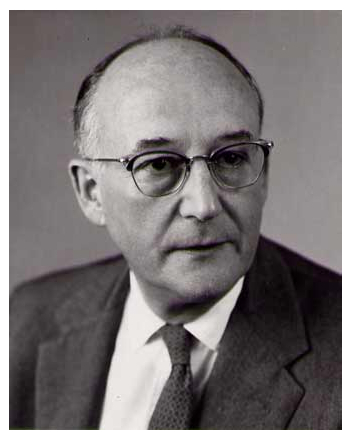
\includegraphics[scale=0.5]{images/morris.jpg}
  \caption{Charles William Morris (1901-1979)}
  \label{morris}
\end{figure}

One of the founders of semiotics, Charles William Morris, has identified the following important notions:

\begin{itemize}
\item \emph{Syntax}~--- relations between the signs of sign system themselves.
\item \emph{Semantics}~--- relations between a sign system and objects.
\item \emph{Pragmatics}~--- relations between a sign system and a person.
\end{itemize}

In a narrower context of programming languages syntax denotes the form of program representation, semantics~--- the ``meaning'' of programs, and pragmatics~---
the relation between programming language and developer. In our course we focus mainly on syntax and semantics, putting all pragmatics questions aside.

\section{Syntax}

Similarly to natural languages, the syntax of a programming language can be decomposed into a few levels (lexical structure, grammar, etc.) However,
unlike natural languages, which have been evolving more or less spontaneously, the syntax for a programming language is intelligently designed taking
into account a number of specific requirements; in particular, it is (as a rule) \emph{unabiguous} and allows for efficient analysis.

To illustrate the concept of programming language syntax consider the following simple snippet in \textsc{C}:

\begin{figure}[h]
  \centering
  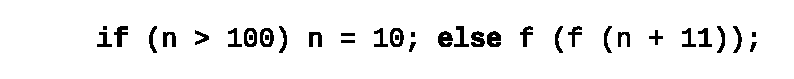
\includegraphics[scale=0.7]{images/01-01.eps}
\end{figure}

From the \emph{lexical} standpoint this fragment can be seen as a sequence of \emph{tokens} (a keyword, a delimiter, an identifier, a binary operator,
a decimal constant, etc.):

\begin{figure}[h]
  \centering
  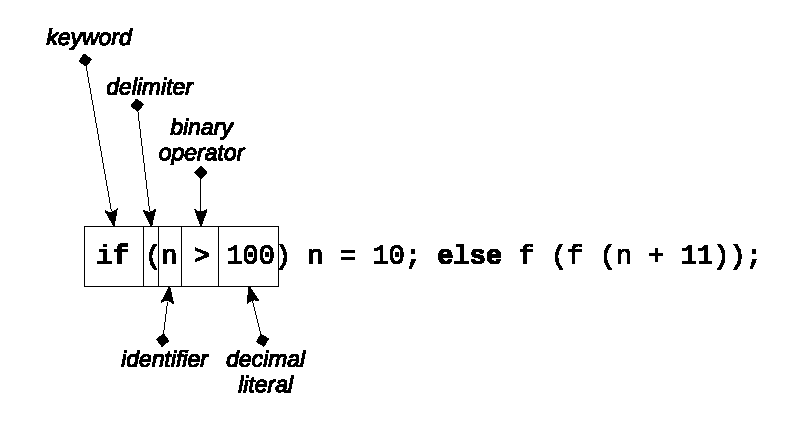
\includegraphics[scale=0.7]{images/01-02.eps}
\end{figure}

This sequence of tokens, in turn, is grouped into an hierarchy of syntactic constructs (in this case, expressions and operators):

\begin{figure}[h]
  \centering
  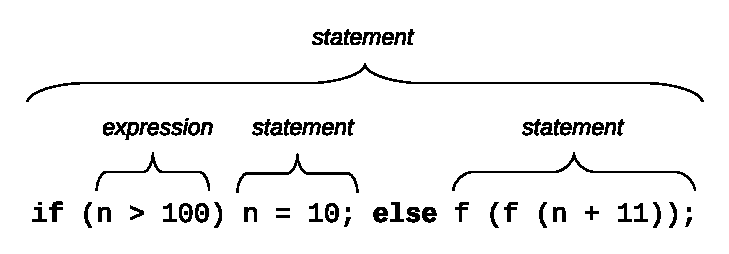
\includegraphics[scale=0.7]{images/01-03.eps}
\end{figure}

Natural languages, as a rule, are \emph{ambiguous}. Consider the following phrase: ``Entering the doors with pets hold them.`` Hold what? The doors or the pets?
In this case we encounter a \emph{global ambiguity} which cannot be resolved even taking into account the context. The only way to resolve it is to
rephrase (``Entering the doors hold your pets'' or ``Hold your pets while entering the doors''). The presence of such unresolvable ambiguities in a
programming language is inacceptable.

\section{Semantics}

The drastic difference between natural and programming languages manifests itself in a full bloom on the semantic level. Unlike natural languages,
for programming languages there are ways to formally specify their semantics and acquire a \emph{mathematically proven} results.

Why formal semantics matters? While in a common practice of using programming languages for application-level software we can rely on our vague, fuzzy
understanding of the meanings of their constructs, when we develop system-level programming \emph{tools}, in particular, compilers, this understanding
turns out to be insufficient. Imagine, for example, that we know that in some programming language expressions consist of variables, constant and four
arithmetic operators. Is this knowledge is complete?

Let us have the following expressions:

\begin{lstlisting}
   0*(x/0)
   1+x-x  
\end{lstlisting}      

What should be the results of their evaluation?

In the first sample, on one hand, the multiplication to zero always gives zero; on the other hand, the division by zero is undefined. So, would the result of
the expression be zero or undefined?

In the second sample, we add a value of \lstinline|x| to \lstinline|1| and immediately subtract it. On one hand this would give us \lstinline|1|; on the
other hand, the value of \lstinline|x| can be undefined, or adding \lstinline|x| to \lstinline|1| might lead to an overflow. So it remains unclear if we
can replace \lstinline|1+x-x| with \lstinline|1| while preserving the behaviour of the program in all cases.

Even if we cannot come up with definite oral answers to these questions we still can write programs using this language; after all, we always can
see what happens in each case if we have a compiler. But what should we do if our task is to implement the \emph{first} compiler for this language?
What happens if we ask a dozen of people to implement a dozen of compilers independently? Whould all these compilers agree in their semantics, or, perhaps, we
eventually will have a dozen of \emph{different} compilers since their authors have \emph{different} intuition? 

One may argue that all these samples come from a very rare and unrealistic use cases. Indeed, how often a new compiler is created, let alone a
dozen of ones? And those snippets with ``murky'' semantics look like antipatterns: why on earth a sane developer whould write ``\lstinline|0*(x/0)|''
instead of ``\lstinline|0|'' or ``\lstinline|1+x-x|'' instead of ``\lstinline|1|''?

The answer, somewhat unexpected, is that actually all these cases are rather \emph{general} then exceptional. Of course, implementing a completely new compiler from scratch is not an
everyday task; however, at the same time programming languages and compilers are rarely developed ``once and for all''. As a rule, both languages
and their compilers evolve through time: new constructs are being added to languages, and new features are being implemented in compilers. Carrying out all of
these routine tasks require a strong semantic foundations. Besides this, compilers by no means are the only semantic-sensitive development instruments:
there is an abundance of other important tools like IDEs, model checkers, static analyzers, debuggers, profilers, etc., all of which have to interpret the
semantics of programs in a coherent way.

Then, not all programs are written directly by human beings. Actually, a fair share of them are generated by other tools, in particular, \emph{preprocessors}
or other \emph{metaprogramming} tools. The results of metaprogramming as a rule look exactly like the samples discussed above: they contain a lot
of vacuous use of constructs and programming language features, and it is \emph{expected} from the underlying compiler to clean up this mess
in a semantics-preserving manner.

Finally, for a compiler there is nothing ``weird'' in those code samples. The reason is simple: compilers do not have intuition. They just 
routinely convert program texts into executables no matter how weird they would look from a human being point of view. To illustrate this,
consider the following short program in \textsc{C}: 

\begin{lstlisting}[language=cc]
m(f,a,s)char*s;
{char c;return f&1?a!=*s++?m(f,a,s):s[11]:f&2?a!=*s++?
1+m(f,a,s):1:f&4?a--?putchar(*s),m(f,a,s):a:f&8?*s?
m(8,32,(c=m(1,*s++,"Arjan Kenter. \no$../.\""),
m(4,m(2,*s++,"POCnWAUvBVxRsoqatKJurgXYyDQbzhLwkNjdMT"
"GeIScHFmpliZEf"),&c),s)):65:(m(8,34,"rgeQjPruaOnDaP"
"eWrAaPnPrCnOrPaPnPjPrCaPrPnPrPaOrvaPndeOrAnOrPnOrPn"
"OaPnPjPaOrPnPrPnPrPtPnPrAaPnBrnnsrnnBaPeOrCnPrOnCaP"
"nOaPnPjPtPnAaPnPrPnPrCaPnBrAnxrAnVePrCnBjPrOnvrCnxr"
"AnxrAnsrOnvjPrOnUrOnornnsrnnorOtCnCjPrCtPnCrnnirWtP"
"nCjPrCaPnOtPrCnErAnOjPrOnvtPnnrCnNrnnRePjPrPtnrUnnr"
"ntPnbtPrAaPnCrnnOrPjPrRtPnCaPrWtCnKtPnOtPrBnCjPronC"
"aPrVtPnOtOnAtnrxaPnCjPrqnnaPrtaOrsaPnCtPjPratPnnaPr"
"AaPnAaPtPnnaPrvaPnnjPrKtPnWaOrWtOnnaPnWaPrCaPnntOjP"
"rrtOnWanrOtPnCaPnBtCjPrYtOnUaOrPnVjPrwtnnxjPrMnBjPr"
"TnUjP"),0);}
main(){return m(0,75,"mIWltouQJGsBniKYvTxODAfbUcFzSp"
"MwNCHEgrdLaPkyVRjXeqZh");}
\end{lstlisting}

If you have any doubts if this is a valid \textsc{C} program, compile and run it. \textsc{C} is never considered as particularly hard to
understand or syntactically challenging (both arguable), yet the program presented is totally incomprehendible. Actually, it
was specifically designed to be such: there is a whole competition in writing \emph{obfuscated}
code\footnote{https://www.cise.ufl.edu/$\tilde\,$manuel/obfuscate/obfuscate.html}. For us, however, the important observation is that this
program no more obfuscated for a compiler as any other one. Our job as compiler implementors is to make them behave is such a way.


\section{The Essence of Translation}

\emph{Translation} is a syntactic transformation of programs in one language into (equivalent) programs into another.
The feasibility of fully automatic translation constituties a drastic difference between programming languages and natural ones.
Although natural language translation techniques and tools made a tremendous progress in a recent years the adequacy of the results
remains the matter of discusstion; and, anyway, this adequacy can not be mathematically proven. For compilers this problem
is essentially solved.

A compiler itself is not a magical creature~--- it is a \emph{program}, written, in turn, in some programming language. Thus, speaking
about compilation, we actually deal with \emph{three} languages:

\begin{figure}[h]
  \centering
  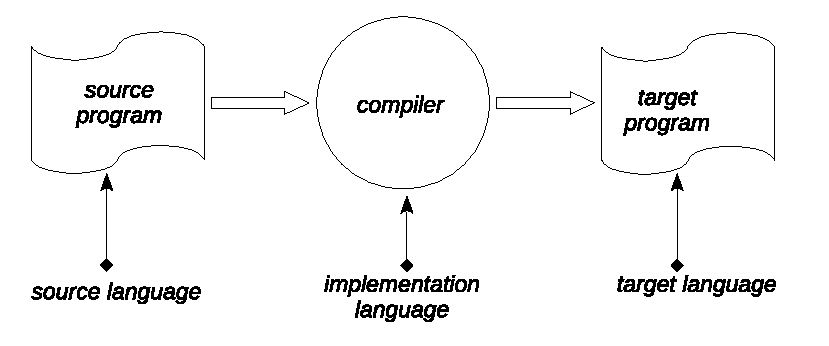
\includegraphics[scale=0.7]{images/01-04.eps}
\end{figure}

\begin{itemize}
\item The language in which the programs being compiled are written (\emph{source language}).
\item The language in which the programs being compiled are compiled (\emph{target language}).
\item The language in which the compiler from source to target language is written (\emph{compiler implementation language}).
\end{itemize}

\section{Translation Subspecies}

As you probably know, there is a subdivision of languages into high- and low-level. This subdivision is not absolute: for example,
\textsc{Haskell} is considered by many as more high-level language than \textsc{C}, which, in turn, is of higher level then \textsc{Fortran}, etc.
As a rule, high-level languages are equipped with type systems, while low-level are not (but \textsc{Scheme} is untyped while there 
exist typed assemblers). This coarse-grained classification of languages leads to a corresponding coarse-grained classification of
translators:

\begin{figure}[h]
  \centering
  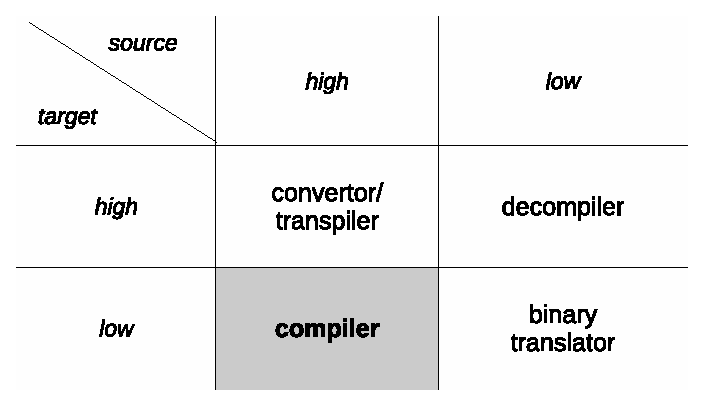
\includegraphics[scale=0.7]{images/01-05.eps}
\end{figure}

There is a somewhat common knowledge that among all these subspecies compilers are the most challenging to implement. While
we generally agree, it's worth mentioning that the other kinds of translators are not pieces of cakes at all: for example,
it is expeccted from a decompiler or convertor to properly utilize the abstractions of the target language, to produce a
human-readable maintanable results, etc.

\section{Environments and Cross-Compilation}

Programs are rarely work in isolation; as a rule they rely on a certain environment: operation system, system- and user-level
libraries, etc. Since compiler is a program itself, it also requires a certain environment, called \emph{compilation environment}.
On the other hand, the environment for which compiler generates its output is called \emph{target environment}. Usually that two
coinside~--- for example, out \lama compiler works under Linux on x86 processor, and generates programs which work
under Linux on x86.

However, in general case, compilation environment can be different from the target one. In this case the compiler is called
\emph{cross-compiler}. For example, we could rewrite our \lama compiler into a cross-one, which, still running on x86,
would generate code for ARM. 

A typical scenario for cross-compilation is \emph{bootstrapping} (see below) or the development of embedded systems when
the target platform is not enough performant/well-equipped to support the execution of a compiler.

\section{Bootstrapping}

An interesting (and practically important) operation involving compilers is their \emph{bootstrapping}. This term denotes the
implementation of a compiler in its own source languages (i.e. when implementation language coinsides with the source one).
The term itself originates from an idiom describing a process of pulling oneself up by the hooks on the back of their own
boots.

\begin{figure}[h]
  \centering
  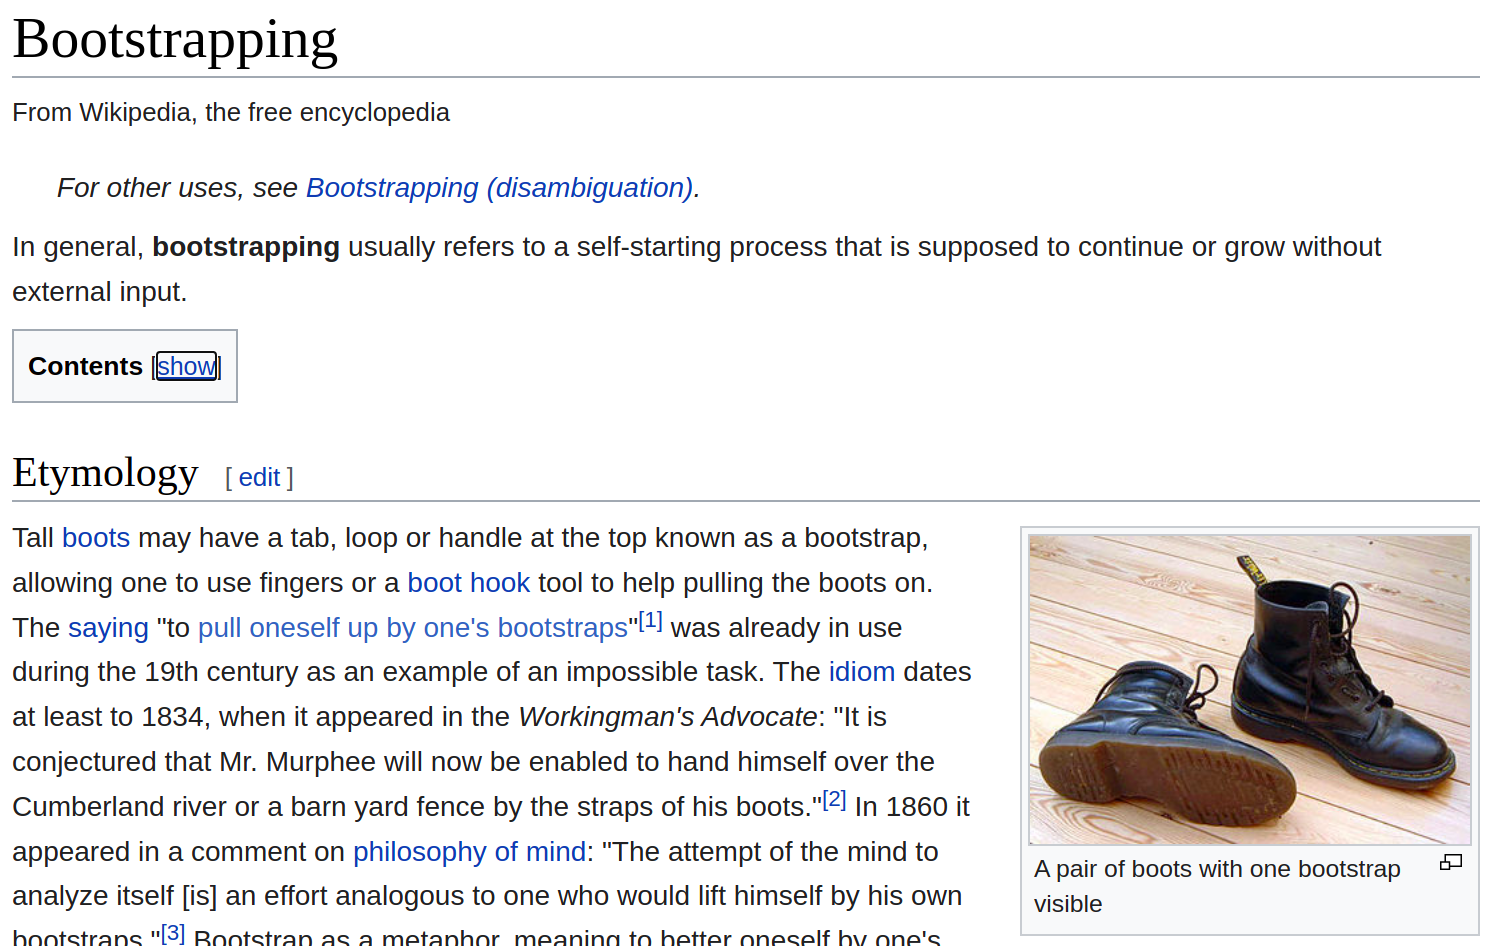
\includegraphics[scale=0.2]{images/bootstrapping.png}
\end{figure}

The bootstrapping of a compiler for a new language (for which no compiler yet exists) is compised of its implementation
in some other language and then rewriting it in this new language using just written compiler. For example, in such a way the \lama compiler was
acquired (\textbf{not really yet}): initially it was implemented in \textsc{OCaml} and then reimplemented in
\lama itself.

If some compiler for the language of interest already exists, but works on some other platform, then it is possible for
implement a \emph{cross-compiler} which works on that platform but generates code for the platform of interest. Then
this compiler can be compiled by itself~--- this is the conventional way, for example, to port \textsc{GCC} compilers
to other platforms.

Finally, if nothing useful exists beside the assembler for the platform of interest, then this assembler itself can be
used to implement a small subset of the desirable language; then this subset can be used to implement a wider subset, and so on.
This is how modern compiler/language zoo was built historically.

Compiler bootstrapping is an ideologically important step: first, it assesses the expressivenes of the language; second, ir witnesses the
maturity of the compiler, since for a new language its compiler, as a rule, is the first large and complex program.

\section{Complete vs. Partial Correctness}

Compiler (as any other translator) has to syntactically transform a program in one language into a program in another, preserving its semantics.
In practice, however there are some subtleties.

Let us have a program $p$. We denote by

\[
x\xrightarrow{\displaystyle{p}} y
\]

the fact that $p$ on input $x$ terminates with the output $y$ (as we know, there may be two other outcomes: $p$ crashes on input $x$ or
$p$ loops forever on input $x$). 

Let us have a compiler, let $source$ be some source program, and let $target$ be a target program after the compilation.
We will say, that a compiler is \emph{complete correct}, iff for arbitrary $source$-$target$ pair and arbitrary
input-output pairs $x$ and $y$

\[
x\xrightarrow{\displaystyle{source}}y \Longleftrightarrow x\xrightarrow{\displaystyle{target}}y
\]

In other words, the behaviour of the source and compiled programs is indistinguishable: on the same input both either
terminate with the same results, or crash/loop.

Consider, however, the following simple program:

\begin{lstlisting}[language=cc]
   # include <stdio.h>

   static int d = 0;

   int main (int argc, char *argv[]) {
     int x;

     x = argc / d;
    
     return 255;
   }  
\end{lstlisting}

A brief analysis reveals that this program has to crash on each input. Indeed, the variable ``\lstinline[language=cc,basicstyle=\normalsize]|d|'' has initial value zero and cannot
be reassigned elsewhere (due to ``\lstinline[language=cc,basicstyle=\normalsize]|static|'' storage class), and division by zero gives a runtime error. We could, alternatively,
try to compile this program with ``\texttt{gcc -O0}'' command and see that it, indeed, crashes.

On the other hand, a more careful analysis shows that the value of the variable ``\lstinline[language=cc,basicstyle=\normalsize]|x|'', during the computation
of which the error occurs, actually is never used, so its computation can be completely omitted. And, indeed, if we compile this program with the command ``\texttt{gcc -O3}'',
it terminates successfully with return code 255! This is because the option ``\texttt{-O3}'' turns on the optimizations, and one of those~--- \emph{dead code elimination}~---
does exactly what we envisioned.

Thus, we can see that in practice target programs not always completely equivalent to the source ones: they can deliver some results on inputs, for which the source
ones loop or crash. This property is called \emph{partial correctness}, and can be formally specified as follows: for arbitrary input-output values $x$ and $y$, and for
arbitrary source and target programs $source$ and $target$

\[
x\xrightarrow{\displaystyle{source}}y \Longrightarrow x\xrightarrow{\displaystyle{target}}y
\]

This means, that when the source program terminates with a definite result, the target also does so with the same result; however, the target one can still deliver some output
values for inputs on which the source program is not defined. In other words, compilers are allowed to \emph{extend the domains} of programs they compile. The
majority of compilers (and other tools as well) are partially correct.

\section{Compiler Architecture}

The majority of real compilers share the same architectural features. They consist of a number of \emph{passes}, each of which
takes on input and returns as a result a certain \emph{intermediate represetation}, \emph{IR}, (not neccessarily the same) of a program
being compiled. The concrete set of these passes and concrete forms of intermediate representations vary from a compiler to a compiler,
but there are still some common representation which can be found throuhout various implementations: \emph{abstract syntax tree},
\emph{three-address code}, \emph{stack machine code}, \emph{static single assignment} (SSA), etc. Some of these forms of representation
will be utilized in our compiler, some others will be left out unused.

All the diversity of passes can be subdivided in a few categories.

\begin{figure}[h]
  \centering
  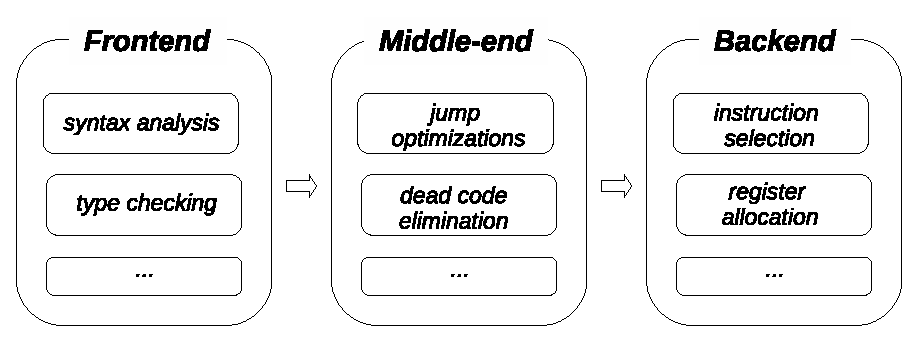
\includegraphics[scale=0.7]{images/01-06.eps}
\end{figure}

First, the \emph{frontend} of a compiler collects a number of \emph{analyzing} passes: syntax analysis, type inference/checking,
name resolution, etc.

Then, the \emph{backend} of a compiler contains code generation passes: instruction selection, register allocation,
instruction scheduing, low-level optimizations.

Finally, there can be \emph{middle-end}, which comprised of various machine-independent optimising passes such as
jump optimizations, dead code elimintation, loop invariant code motion, common subexpression elimination, etc.

Most compilers allow to peep on what's going on under the hood. For example, \texttt{GCC} accepts the
option \texttt{-ftime-report}, which makes it output the time taken by each pass performed. An example
of such an output is shown below:

\begin{scriptsize}
\begin{verbatim}
Execution times (seconds)
 phase setup             :   0.00 ( 0%) usr   0.00 ( 0%) sys   0.00 ( 0%) wall    1179 kB (25%) ggc
 phase parsing           :   0.03 (33%) usr   0.01 (100%) sys   0.04 (40%) wall    1197 kB (25%) ggc
 phase opt and generate  :   0.06 (67%) usr   0.00 ( 0%) sys   0.06 (60%) wall    2328 kB (49%) ggc
 callgraph optimization  :   0.01 (11%) usr   0.00 ( 0%) sys   0.00 ( 0%) wall       0 kB ( 0%) ggc
 cfg cleanup             :   0.00 ( 0%) usr   0.00 ( 0%) sys   0.01 (10%) wall       0 kB ( 0%) ggc
 trivially dead code     :   0.00 ( 0%) usr   0.00 ( 0%) sys   0.01 (10%) wall       0 kB ( 0%) ggc
 df reaching defs        :   0.01 (11%) usr   0.00 ( 0%) sys   0.00 ( 0%) wall       0 kB ( 0%) ggc
 alias analysis          :   0.01 (11%) usr   0.00 ( 0%) sys   0.00 ( 0%) wall      55 kB ( 1%) ggc
 preprocessing           :   0.00 ( 0%) usr   0.00 ( 0%) sys   0.01 (10%) wall     345 kB ( 7%) ggc
 lexical analysis        :   0.03 (33%) usr   0.01 (100%) sys   0.01 (10%) wall       0 kB ( 0%) ggc
 parser inl. func. body  :   0.00 ( 0%) usr   0.00 ( 0%) sys   0.02 (20%) wall      79 kB ( 2%) ggc
 dominator optimization  :   0.00 ( 0%) usr   0.00 ( 0%) sys   0.01 (10%) wall      45 kB ( 1%) ggc
 forward prop            :   0.01 (11%) usr   0.00 ( 0%) sys   0.00 ( 0%) wall      13 kB ( 0%) ggc
 loop init               :   0.02 (22%) usr   0.00 ( 0%) sys   0.01 (10%) wall     193 kB ( 4%) ggc
 loop fini               :   0.00 ( 0%) usr   0.00 ( 0%) sys   0.01 (10%) wall       0 kB ( 0%) ggc
 final                   :   0.00 ( 0%) usr   0.00 ( 0%) sys   0.01 (10%) wall      48 kB ( 1%) ggc
 TOTAL                 :   0.09             0.01             0.10               4714 kB
\end{verbatim}
\end{scriptsize}

\section{The \lama Compiler}

Now, when we discussed a little bit how compilers work, let's have a look at \lama compiler, which will be our main
tool throuhgout the course, and which we will be implementing.

The \lama compiler is organized much simpler than the majority of industrial-tier compilers like \texttt{GCC}, which we already
mentioned multiple times (see Fig.~\ref{lama-comp}).

\begin{figure}[t]
  \centering
  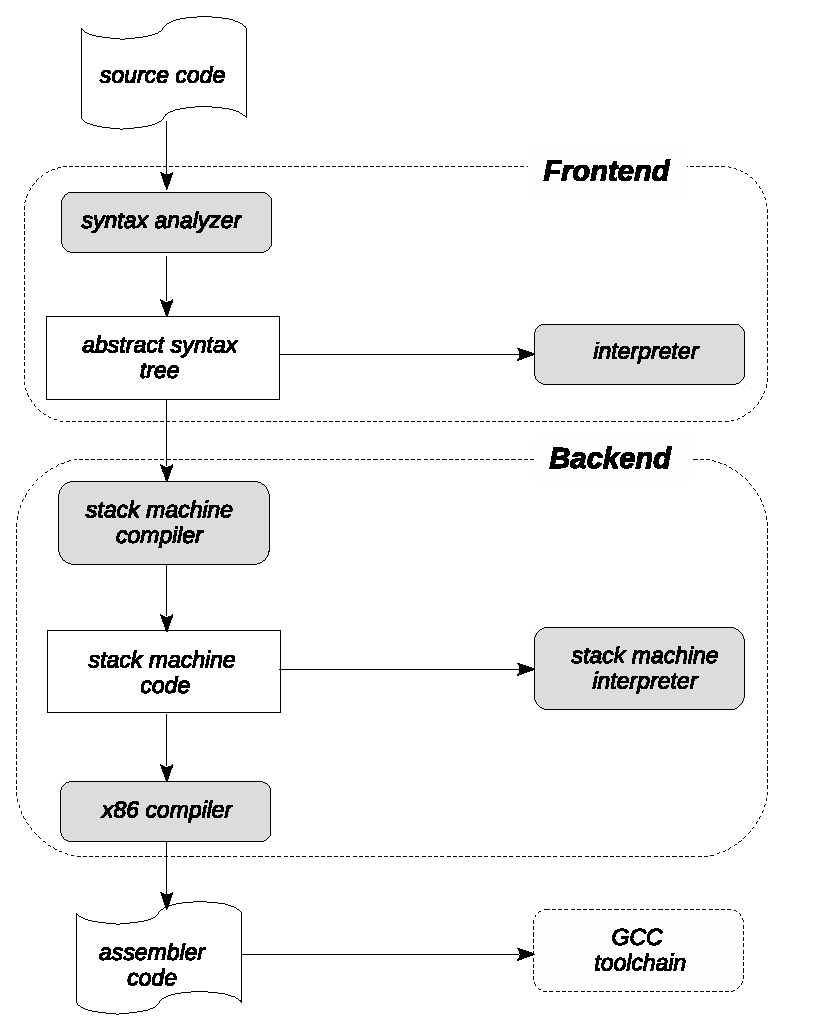
\includegraphics[scale=0.7]{images/01-07.eps}
  \caption{The Structure of \lama Compiler}
  \label{lama-comp}
\end{figure}


The source file with a \lama program is parsed by a syntax analyser which converts it into an
abstract syntax tree, or AST. AST is one of the most important program representations, and its use in compilers and other
tools is ubiquitious.

The next component, which is rarely implemented in real-world compilers, is a source-level \emph{interpreter}. We
consider this object in details later, for now it is sufficient to know that interpreter is a component which
directly runs a program in some representation~--- in our case, in the form of AST,~--- according to the semantics of the language. 
The presence of interpreter plays an important role from both educational and technological standpoints. First,
the implementation of interpreter facilitates the internalization of formal semantics description method which
we use, namely~--- big-step operational semantics. Next, it allows to find and eiminate some errors 
at early stage. The implementation of interpreter is rather a simple task, and it is advantageous to be capable of running program
at early stages of compiler implementation.

Then, there is a compiler of AST into \emph{stack machine} code. This machine resembles a simplified model of
actual hardware processor; thus, on one hand, to generate stack machine code a similar set of tasks has to be
solved; on the other, these solutions are a bit simpler than for an actual hardware. Generated stack machine
code can then be run on the \emph{stack machine interpreter}. Similarly to source-level interpreter case,
the capability to run stack machine code makes it possible to develop and debug stack machine compiler
in isolation.

Finally, the last component of the compiler is code generator for \texttt{x86} processor which
transforms stack machine code into \texttt{x86} assembler program; this program is then passed to
the \textsc{GCC} infrastructure to be finally transformed into an object module.

Thus, from the architectural point of view, syntax analyser constitutes a fronted, while compilers for
stack machine and \texttt{x86}~--- a backend.

\end{document}

